% ===========================================================================
% Extended version: appendix (not part of the DAC submission; hosted with the code)
% ===========================================================================
\onecolumn
% In this one-column appendix a table is not a float: it is set where it is input, right before the text that cites
% it, and cannot be separated from the first line of that text, so a table and its citation always share a page.
\makeatletter
\let\CA@table\table \let\CA@endtable\endtable
\renewenvironment{table}[1][]{\par\addvspace{\intextsep}\noindent\begin{minipage}{\linewidth}\def\@captype{table}}%
  {\end{minipage}\par\nopagebreak\vskip\intextsep}
\let\CA@figure\figure \let\CA@endfigure\endfigure
\renewenvironment{figure}[1][]{\par\addvspace{\intextsep}\noindent\begin{minipage}{\linewidth}\def\@captype{figure}}%
  {\end{minipage}\par\nopagebreak\vskip\intextsep}
\makeatother
\section*{Appendix}
\addcontentsline{toc}{section}{Appendix}
This appendix accompanies the anonymous repository. It documents every design decision of the study, gives
complete results that do not fit the page limit, and answers the questions we expect from reviewers. Section
numbers refer to the main paper. \Cref{fig:retrieval} breaks the retrieval of \cref{tab:main} down per rewrite family
and shows it as a candidate list (recall@$k$).

\renewcommand{\thesubsection}{\Alph{subsection}}
\FloatBarrier
\begin{figure}[h]
\centering
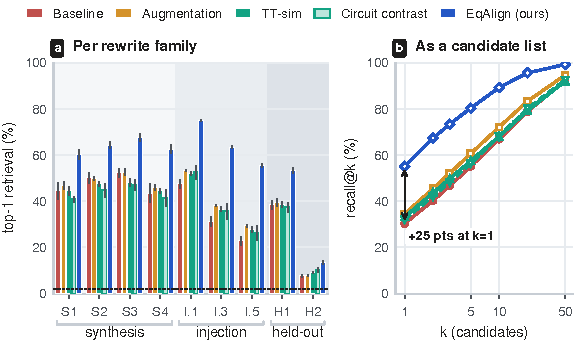
\includegraphics[width=0.6\textwidth]{figs/fig_retrieval.pdf}
\caption{\textbf{Retrieval on EPFL.} (a) Top-1 retrieval of the proven equivalent per family (mean $\pm$ s.d.\
over 5 seeds; dashed: chance). (b) Recall@$k$ among the $k$ most similar original gates, pooled over all restructured
pairs of the 7 fixed families (5-seed mean), so large circuits weigh more than in Top-1, which averages circuits.}
\label{fig:retrieval}
\end{figure}
\subsection{Reproducibility}\label{app:repro}
\noindent\textbf{Environments.} The models of the main text (\cref{tab:main}, \cref{fig:audit,fig:twolevel}, RQ1 and RQ2,
ISCAS, widths 64 and 256, all GPU experiments) were trained on 8 NVIDIA RTX~6000 Ada GPUs with Python~3.11 and
PyTorch~2.7.1. The protocol was developed, and first run in full, on a 2-core x86 CPU with 7\,GB of memory and no GPU
(Python~3.13, PyTorch~2.15); the confirmatory evaluation (made once, on that run's models) and the timings of
\cref{fig:sweep}b come from that run, and the external audits were run there. \textbf{Cross-environment check.} Before any new experiment, the GPU machine retrained the CPU run's exact
setting (7 regimes, 3 seeds) and compared 70 metrics with tolerances fixed in advance; 68 have a CPU value and 67 of them agree (the two without are the
$L_1$ regimes' worst-case ratios, which the CPU run did not compute). The exception is
circuit-level contrast's $\rho$ under injection (CPU 0.94, GPU 1.08): over all families its inconsistency is unchanged
(0.0281 against 0.0283), but on injected pairs its error falls by about 7\% and its inconsistency rises by about 6\%,
which together move the ratio; a CPU rerun with the GPU code gives 1.06, and the training losses differ
from the first epoch, which points to the PyTorch versions rather than GPU arithmetic. \textbf{Software.} Both environments use aigverse~0.1.7~\cite{aigverse} (Python bindings for the EPFL logic synthesis libraries
\cite{DBLP:journals/corr/abs-1805-05121}: mockturtle, kitty, lorina),
PySAT with CaDiCaL~1.5.3~\cite{DBLP:conf/sat/IgnatievMM18,cadical2020}, NumPy, SciPy and scikit-learn. Every number computed from our runs is
written to the \texttt{numbers*.tex} files by the scripts that \texttt{build.sh} calls (\texttt{make\_numbers2.py} first); tables and figures are generated by
\texttt{make\_tables.py}, \texttt{make\_general.py}, \texttt{make\_appendix.py} and \texttt{make\_figs2.py}.

\begin{table}[h]
\centering
\caption{Pipeline stages and wall time on a 2-core CPU (training times measured with other jobs running concurrently).}
\label{tab:app_pipeline}
\small
\begin{tabular}{lll}
\toprule
Stage & Script & Time \\
\midrule
Cone extraction (EPFL) & \texttt{data.py} & 11\,s \\
Fixed variants and certification (EPFL) & \texttt{data.py} & 7\,min \\
Adversarial variants, 16 per circuit & \texttt{evaluate.py} & 29\,min \\
SAT-proven matching of all EPFL pairs & \texttt{rematch.py} & 43\,s ($\approx10^6$ SAT calls) \\
Held-out variants H1, H2 (EPFL) & \texttt{heldout\_run.py} & 9\,min \\
ISCAS circuits, variants and matching & \texttt{iscas\_run.py} & see log \\
Training: Baseline (12 epochs) & \texttt{train.py} & 4\,min \\
Training: Augmentation (12 epochs) & \texttt{train.py} & 7\,min \\
Training: \ours (12 epochs) & \texttt{train.py} & 7\,min \\
Training: TT-sim (12 epochs) & \texttt{train.py} & 9\,min \\
Training: Circuit contrast (12 epochs) & \texttt{train.py} & 9\,min \\
Training: Bidirectional baseline (12 epochs) & \texttt{train.py} & 13\,min \\
\bottomrule
\end{tabular}
\end{table}

\noindent\textbf{Pipeline and run time.} \Cref{tab:app_pipeline} lists every stage with its script and wall time.

\noindent\textbf{Seeds.} Data generation uses fixed seeds (cones: 0; test variants: $10{,}000+n$; adversarial:
$777+n$; held-out H2: $50{,}000+n$; ISCAS: 2027 and $20{,}000+n$). Training seeds are 0 to 4 in the GPU run and 0 to 2 in the CPU run. The validation
split is a fixed permutation (seed 12345) of the training circuits.

\FloatBarrier
\subsection{Rewrite Families in Detail}\label{app:families}
\begin{table}[h]
\centering
\caption{Rewrite families. Pass names refer to mockturtle via aigverse; parameters not listed are library defaults.}
\label{tab:app_families}
\small
\begin{tabular}{p{2.3cm}p{10.4cm}p{3.6cm}}
\toprule
Family & Definition & Used for \\
\midrule
S1 & cut rewriting; resubstitution; balancing (SOP); SOP refactoring & train, test \\
S2 & balancing; cut rewriting (zg); SOP refactoring (zg); resubstitution (10 leaves, 3 inserts) & train, test \\
S3 & SOP refactoring; cut rewriting; cut rewriting (zg) & train, test \\
S4 & resubstitution (10 leaves, 3 inserts); balancing; cut rewriting; resubstitution & train, test \\
I.$r$ & each gate rebuilt with probability $r$ by one of three identities ($(x\wedge y)\wedge(x\vee y)$, Shannon expansion on a random earlier signal, $(x\wedge y)\wedge\neg((x\wedge y)\wedge\neg x)$), chosen uniformly & train ($r=0.15,0.3$), test ($r=0.1,0.3,0.5$) \\
H1 & resubstitution with don't cares (window 12, 10 leaves); balancing (ESOP); cut rewriting with don't cares (zg); SOP refactoring with don't cares and reconvergence-driven cuts & test only \\
H2 & each gate rebuilt with probability 0.3 as $(x\oplus y)\oplus(x\vee y)$, XOR built from three ANDs & test only \\
Adversarial & with prob.\ 0.5: 1 to 4 random passes from S-type passes, then with prob.\ 0.5 injection $r\sim U(0.02,0.15)$; otherwise injection $r\sim U(0.02,0.2)$ with 1 to 3 identity types; rejected if gate count grows by $>30\%$; 16 per circuit & test only \\
\bottomrule
\end{tabular}
\end{table}

\Cref{tab:app_families} gives the exact passes, their parameters, and the resulting size changes. Synthesis
passes are applied in order, each followed by dangling-node cleanup. ``zg'' denotes zero-gain replacements
(\texttt{allow\_zero\_gain}), which change structure without reducing size.

\noindent\textbf{Why these families.} Synthesis is the realistic case: it is what a deployed model meets.
Injection is a controlled stress test whose intensity $r$ we can dial; it is reported separately so that it
cannot inflate the synthesis results. H1 and H2 test generalization to rewrites \emph{not} seen in training: H1
changes the passes (don't-care based, ESOP balancing) but stays close to synthesis; H2 changes the local
identity, re-expressing an AND through XORs. Adversarial variants approximate a worst case within a realistic
size budget (at most 30\% growth); we sample rather than optimize them, so the reported worst case is a lower
bound on the true worst case.

\noindent\textbf{Excluded circuits.} Two EPFL test circuits (indices 316 and 338) make mockturtle's
don't-care passes abort with a memory error; we isolate each circuit in its own process and exclude these two
from H1/H2 only. ISCAS circuits that fail in the same way are listed in the released logs.

\FloatBarrier
\subsection{Certification and Matching}\label{app:matching}
\noindent\textbf{Output certification} uses \texttt{equivalence\_checking} of mockturtle (a SAT miter with
functional reduction) with \texttt{conflict\_limit=0} (no limit); a variant is kept only if the call returns
\emph{equivalent}. No variant was rejected and no call was undecided.

\begin{figure}[h]
\centering
\begin{minipage}{0.92\textwidth}
\hrule\smallskip
\textbf{Algorithm 1} SAT-proven gate matching between $G$ and its variant $G'$\smallskip\hrule\smallskip
\begin{tabbing}
\quad\=\quad\=\quad\=\kill
\textbf{Input:} $G$, $G'$ with shared PIs; $N=4{,}096$ random input patterns\\
1:\>Simulate both circuits on the $N$ patterns; canonical signature $\sigma(w)$ = signature, complemented if its first bit is 1\\
2:\>$B\leftarrow$ buckets of the gates of $G$ by $\sigma$\\
3:\>Tseitin-encode $G$ and $G'$ into one incremental SAT instance with shared PI variables\\
4:\>\textbf{for} each AND gate $u$ of $G'$ \textbf{do}\\
5:\>\>\textbf{for} each $v\in B[\sigma(u)]$ in topological order \textbf{do}\\
6:\>\>\>$\pi\leftarrow[\,\text{signatures of } v \text{ and } u \text{ differ}\,]$; add $t\Rightarrow(x_v\oplus x_u\oplus\pi)$ for a fresh $t$\\
7:\>\>\>\textbf{if} \textsc{Solve}(assume $t$) = UNSAT \textbf{then} record $(v,u,\pi)$; disable $t$; \textbf{break}\\
8:\>\>\>\textbf{else} disable $t$ \quad\emph{(a counterexample: $u$ and $v$ differ)}\\
\textbf{Output:} proven pairs $(v,u,\pi)$ with $f_u=f_v\oplus\pi$
\end{tabbing}
\hrule
\end{minipage}
\caption{Matching procedure. Every recorded pair carries a SAT proof; signature agreement alone is never accepted.}
\label{alg:match}
\end{figure}

\noindent\textbf{Gate matching} (\cref{alg:match}). The two circuits are Tseitin-encoded once into one
incremental CaDiCaL instance with shared PI variables. For a candidate $(v,u,\pi)$ we add a fresh activation
literal $t$ with clauses $t\Rightarrow (x_v\oplus x_u\oplus\pi)$ and solve under assumption $t$; UNSAT proves
$f_u=f_v\oplus\pi$, after which $t$ is permanently disabled.

\begin{table}[h]
\centering
\caption{Simulation-only matching versus SAT (EPFL test set). Candidates: variant gates with a signature-matching original gate; false: no candidate is equivalent; near-constant: share of false matches with $\min(p,1-p)<0.01$.}
\label{tab:app_false}
\small
\begin{tabular}{lrrrr}
\toprule
Family & candidates & false & false (\%) & near-constant (\%) \\
\midrule
S1 & 18,783 & 61 & 0.32 & 51 \\
S2 & 17,836 & 222 & 1.24 & 72 \\
S3 & 21,472 & 336 & 1.56 & 77 \\
S4 & 19,653 & 229 & 1.17 & 77 \\
I.1 & 29,892 & 279 & 0.93 & 93 \\
I.3 & 36,328 & 941 & 2.59 & 96 \\
I.5 & 42,636 & 1,496 & 3.51 & 96 \\
\bottomrule
\end{tabular}
\end{table}

\noindent\textbf{False simulation matches.} \Cref{tab:app_false} breaks down, per family, how many variant gates
have a signature-matching candidate and how many of them have no proven equivalent. Most false matches are
gates that are almost always 0 or 1 ($\min(p,1-p)<0.01$), whose 4{,}096-pattern signatures collapse to (near)
constant vectors; the injection identity $(x\wedge y)\wedge\neg((x\wedge y)\wedge\neg x)$, whose inner gate is constant 0, creates such
gates on purpose.


\noindent\textbf{Why the first proven candidate.} A variant gate may have several equivalent original gates
when the original contains redundancy. Recording the first proven one keeps one label per variant gate. For
retrieval this is conservative: if the nearest original gate is a different but equivalent gate, it counts as a
miss.

\FloatBarrier
\subsection{Metrics: Definitions and Design Choices}\label{app:metrics}
Let $\mathcal P_c$ be the proven pairs of circuit $c$ under one variant, and $\mathcal R_c\subseteq\mathcal P_c$ the
restructured ones. For a family $F$, per-circuit values are averaged over the variants of $F$ and then over circuits:
\begin{align*}
\Delta\mathrm{MAE}&=\tfrac1{|\mathcal P_c|}\textstyle\sum_{(v,u,\pi)\in\mathcal P_c}\big(|\hat p'_u-p'_u|-|\hat p_v-p_v|\big),\\
\rho&=\overline{\textstyle\frac1{|\mathcal R_c|}\sum_{\mathcal R_c}\delta(v,u)}\;\Big/\;\overline{\textstyle\frac1{|\mathcal R_c|}\sum_{\mathcal R_c}|\hat p_v-p_v|},
\end{align*}
where the bars average over circuits; $\rho$ is thus a ratio of averages, which is stable when individual errors
are small. \textbf{Retrieval} uses pairs in $\mathcal R_c$ with $\pi=0$; the candidate set is all AND gates of $G$;
a hit requires $\cos(\mathbf z_v,\mathbf z'_u)>\cos(\mathbf z_w,\mathbf z'_u)$ for all other gates $w$ (pessimistic
ties). \Cref{tab:main} averages hits per circuit; recall@$k$ in \cref{fig:retrieval} pools all pairs, which
weights large circuits more and explains why Top-1 and recall@1 differ. \textbf{AUROC} uses one negative per
positive: a random original gate (AUROC) or a random original gate at the same logic level (AUROC$_\mathrm{lvl}$).
\textbf{Worst case}: for each adversarial variant we compute the matched-gate MAEs of variant and original;
per circuit we keep the variant with the largest difference. \textbf{Noise floor}: for the five seeds
$s\ne s'$ of a regime, the mean of $|\hat p^{(s)}_v-\hat p^{(s')}_v|$ over the restructured original gates of
all fixed families, averaged over seed pairs and circuits.

\noindent\textbf{Why restructured pairs.} With a fanin-only encoder, a gate whose fanin cone is unchanged gets
\emph{exactly} the same prediction in both circuits. Including such pairs would dilute every average with zeros
in proportion to how little a rewrite changes. The bidirectional encoder (\cref{sec:generality}) can move even
unrestructured gates through fanout context, so its table entries use all pairs.

\noindent\textbf{Why a ratio and a noise floor.} $\rho$ answers ``how large is the self-disagreement relative to
the error users already accept?'', but it falls when the error grows. The noise floor answers ``is the
self-disagreement larger than what retraining alone produces?'' and does not depend on the error.

\FloatBarrier
\subsection{Models and Training}\label{app:models}
\begin{table}[h]
\centering
\caption{Hyperparameters (identical for all regimes unless stated).}
\label{tab:app_hparams}
\footnotesize
\begin{tabular}{ll|ll}
\toprule
State size & 64 & Optimizer & Adam, one-cycle cosine, peak $2\times10^{\ensuremath{-}3}$, 10\% warm-up \\
Rounds & 2 & Gradient clipping & global norm 1.0 \\
$\phi,\psi$, projection head $q$ & 2-layer MLP, ReLU & Batch & 16 circuits (32 with variants) \\
Probability head & 2-layer MLP, sigmoid & Epochs & 12 \\
Probability loss & $L_1$ on all AND gates & Seeds & 0 to 4 (CPU run: 0 to 2) \\
\ours\ & InfoNCE, $\tau=0.1$, $\le 512$ pairs/batch & TT-sim & 64 random pairs/circuit, 1{,}024 patterns \\
Circuit contrast & mean-pooled $\mathbf z$, InfoNCE, $\tau=0.1$ & Loss weights & selected on validation (\cref{app:selection}) \\
\bottomrule
\end{tabular}
\end{table}

\noindent\Cref{tab:app_hparams} lists the hyperparameters, identical for all regimes unless stated. Every node starts from a learned state chosen by its type (constant, PI or AND), so all PIs share one initial state and the encoder sees the structure of a fanin cone, not which inputs feed it.

\noindent\textbf{Bidirectional encoder.} Each round first runs the forward pass with attention weights
$\alpha_a,\alpha_b=\mathrm{softmax}(\mathbf w^\top[\mathbf h_v,\mathbf m_a],\,\mathbf w^\top[\mathbf h_v,\mathbf m_b])$
and $\mathbf m=2(\alpha_a\mathbf m_a+\alpha_b\mathbf m_b)+\psi(\mathbf m_a\odot\mathbf m_b)$, then a reverse pass from
the highest level down in which each gate sums messages $\phi_r([\mathbf h_w,c])$ from its fanout gates $w$ and
updates its state with a second GRU, as in DeepGate~\cite{DBLP:conf/dac/0019KSWY022}. It uses the same loss weights as the
unidirectional encoder ($\lambda=\LamStar$) without re-selection, which can only disadvantage \ours.

\begin{table}[h]
\centering\scriptsize
\caption{Encoder size against blindness and repair (EPFL test, 5 seeds each). Recurrent: restructured pairs; transformer:
all proven pairs. $\rho_{\text{H2}}$: range over baseline, augmentation and \ours.}
\label{tab:app_scale}
\resizebox{\columnwidth}{!}{\begin{tabular}{l r cc ccc c}
\toprule
 & & \multicolumn{2}{c}{Baseline} & \multicolumn{3}{c}{Top-1 (\%)} & \\
\cmidrule(lr){3-4}\cmidrule(lr){5-7}
Encoder & Params & $\rho$ Syn. & MAE & Base & Augm. & \ours & $\rho_{\text{H2}}$ (all) \\
\midrule
Recurrent 64 & 46k & 0.85 & 0.0189 & 41.0 & 44.5 & \hl \textbf{63.4} & 5.9 to 7.3 \\
Recurrent 128 & 182k & 0.85 & 0.0185 & 39.4 & 44.9 & \hl \textbf{65.8} & 6.1 to 7.1 \\
Recurrent 256 & 725k & 0.89 & 0.0194 & 39.6 & 45.5 & \hl \textbf{63.7} & 5.8 to 7.3 \\
Recurrent 256, 4 rounds & 725k & 0.89 & 0.0185 & 38.3 & 44.8 & \hl \textbf{67.4} & 5.3 to 7.4 \\
Recurrent 1024 & 11.6M & 0.86 & 0.0192 & 38.4 & 41.7 & \hl \textbf{64.7} & 6.4 to 7.1 \\
\midrule
Transformer 128 & 480k & 0.76 & 0.0197 & 17.5 & 18.8 & \hl \textbf{49.0} & 6.5 to 7.0 \\
Transformer 256 & 1.8M & 0.69 & 0.0217 & 19.3 & 19.3 & \hl \textbf{48.2} & 5.6 to 6.9 \\
Transformer 512 & 7.2M & 0.74 & 0.0236 & 18.9 & 18.8 & \hl \textbf{47.5} & 5.2 to 6.5 \\
\bottomrule
\end{tabular}
}
\end{table}
\noindent\textbf{Model size.} \cref{tab:app_scale} sets blindness against encoder size: over a \ScFold-fold range of recurrent
encoders and a 15-fold range of transformers, the baseline's $\rho$ and retrieval barely move, every regime fails on H2 at
every size, and \ours's lead over the baseline and augmentation holds (on all 7 designs each time). At width 128, as at width 256, \ours\ leads each of the other six regimes by \ScOneTwoEightMin\ to \ScOneTwoEightMax\ points, again on all 7 designs. With 4 propagation rounds instead of 2 at width 256, which widens each gate's receptive field, the baseline's $\rho$ under synthesis is \ScDeepBaseRho\ and its retrieval \ScDeepBaseTop\%, and \ours\ leads each of the other six regimes by \ScDeepLeadMin\ to \ScDeepLeadMax\ points on all 7 designs: depth does not remove the blindness either. Each size was selected by
the main-text rule; for the two largest encoders the learning rate chosen, $2.5\!\times\!10^{-4}$, is the smallest of the grid
fixed in advance ($\{10,5,2.5\}\!\times\!10^{-4}$, below the $5\!\times\!10^{-4}$ that width 256 had chosen), where the next one
is within 4\% in validation MAE and $10^{-3}$ fails to train; at these sizes \ours\ costs no accuracy (MAE within 1\% of the
baseline). We also trained width 512 twice, with the grids $\{20,10,5\}\!\times\!10^{-4}$ and $\{10,5,2.5\}\!\times\!10^{-4}$. Both times the rule chose $10^{-3}$, at which some seeds of several regimes stay at the constant predictor (validation MAE 0.126; all five seeds of circuit contrast), while all ten final runs of \ours\ and of $L_1$ + TT-sim train. Since the means would mix trained and untrained runs, we do not report this width. On ISCAS the recurrent encoder of width 1024 retrieves \ScIsBase\% as baseline and \ScIsOurs\% with \ours.

\FloatBarrier
\subsection{Model Selection and Full Validation Results}\label{app:selection}
\begin{table}[h]
\centering
\caption{All validation results (seed 0) used for selection; \texttt{base\_s0} uses the selected learning rate $2\times10^{\ensuremath{-}3}$, \texttt{base\_lr} rows are the other two candidates.}
\label{tab:app_val}
\small
\begin{tabular}{lrr}
\toprule
Run & val.\ MAE & val.\ Top-1 (\%) \\
\midrule
\texttt{aug\_s0} & 0.0152 & 36.8 \\
\texttt{base\_s0} & 0.0148 & 33.9 \\
\texttt{circ\_ph\_l0.05\_s0} & 0.0148 & 37.7 \\
\texttt{circ\_ph\_l0.2\_s0} & 0.0167 & 39.1 \\
\texttt{circ\_ph\_l0.5\_s0} & 0.0284 & 34.5 \\
\texttt{circ\_ph\_l1\_s0} & 0.0318 & 33.3 \\
\texttt{eqalign\_l0.05\_s0} & 0.0132 & 53.5 \\
\texttt{eqalign\_l0.1\_s0} & 0.0145 & 55.4 \\
\texttt{eqalign\_l0.2\_s0} & 0.0161 & 55.9 \\
\texttt{eqalign\_l0.5\_s0} & 0.0239 & 54.5 \\
\texttt{eqalign\_l1\_s0} & 0.0231 & 57.6 \\
\texttt{eqalign\_l2\_s0} & 0.0286 & 56.3 \\
\texttt{eqalign\_ph\_l0.05\_s0} & 0.0145 & 53.7 \\
\texttt{eqalign\_ph\_l0.1\_s0} & 0.0151 & 57.0 \\
\texttt{eqalign\_ph\_l0.2\_s0} & 0.0166 & 58.7 \\
\texttt{eqalign\_ph\_l0.5\_s0} & 0.0192 & 58.3 \\
\texttt{eqalign\_ph\_l1\_s0} & 0.0218 & 58.5 \\
\texttt{eqalign\_ph\_l2\_s0} & 0.0243 & 58.5 \\
\texttt{l1align\_l0.0003\_s0} & 0.0156 & 37.3 \\
\texttt{l1align\_l0.001\_s0} & 0.0162 & 37.0 \\
\texttt{l1align\_l0.003\_s0} & 0.0168 & 36.6 \\
\texttt{l1align\_l0.01\_s0} & 0.0176 & 34.4 \\
\texttt{l1align\_l0.03\_s0} & 0.1269 & 1.6 \\
\texttt{l1tt\_l0.001\_s0} & 0.0149 & 36.9 \\
\texttt{l1tt\_l0.003\_s0} & 0.0157 & 37.3 \\
\texttt{l1tt\_l0.01\_s0} & 0.0169 & 35.9 \\
\texttt{ttsim\_ph\_l0.03\_s0} & 0.0150 & 34.9 \\
\texttt{ttsim\_ph\_l0.1\_s0} & 0.0148 & 34.8 \\
\texttt{ttsim\_ph\_l0.5\_s0} & 0.0150 & 33.4 \\
\texttt{ttsim\_ph\_l1\_s0} & 0.0149 & 33.1 \\
\texttt{ttsim\_ph\_l2\_s0} & 0.0153 & 32.0 \\
\texttt{base\_lr0.0005\_s0} & 0.0171 & 32.6 \\
\texttt{base\_lr0.001\_s0} & 0.0157 & 33.6 \\
\bottomrule
\end{tabular}
\end{table}

\noindent The rule (highest validation restructured retrieval with validation MAE within 25\% of the baseline)
was applied identically to every loss weight; \cref{tab:app_val} lists every validation result it used. The 25\%
tolerance was fixed when the rule was written; with a 10\% tolerance the rule would select $\lambda=0.1$ for \ours,
whose test results are within one seed-standard-deviation of $\lambda=0.2$ (\cref{tab:ablation}).

\begin{table}[h]
\centering
\caption{All loss weights on validation and test (seed 0), including those the selection rule did not choose.}
\label{tab:app_ablation_full}
\footnotesize\setlength{\tabcolsep}{3pt}
\begin{tabular}{l cc cccc}
\toprule
 & \multicolumn{2}{c}{Validation} & \multicolumn{4}{c}{Test (seen families)} \\
\cmidrule(lr){2-3}\cmidrule(lr){4-7}
Variant & MAE & Top-1 & MAE & $\rho$ & Top-1 & AUROC$_\mathrm{lvl}$ \\
\midrule
Baseline & 0.0148 & 33.9 & 0.0189 & 0.97 & 41.5 & 0.766 \\
Augmentation & 0.0152 & 36.8 & 0.0177 & 0.86 & 44.8 & 0.785 \\
\midrule
\ours\ $\lambda$=0.05 & 0.0145 & 53.7 & 0.0183 & 0.80 & 61.6 & 0.856 \\
\ours\ $\lambda$=0.1 & 0.0151 & 57.0 & 0.0191 & 0.81 & 62.5 & 0.838 \\
\ours\ $\lambda$=0.2$^\star$ & 0.0166 & 58.7 & 0.0228 & 0.70 & 62.2 & 0.844 \\
\ours\ $\lambda$=0.5 & 0.0192 & 58.3 & 0.0258 & 0.72 & 60.9 & 0.858 \\
\ours\ $\lambda$=1 & 0.0218 & 58.5 & 0.0248 & 0.78 & 61.8 & 0.859 \\
\ours\ $\lambda$=2 & 0.0243 & 58.5 & 0.0289 & 0.73 & 61.7 & 0.851 \\
\ours\ no proj., $\lambda$=0.2 & 0.0161 & 55.9 & 0.0244 & 0.85 & 59.6 & 0.831 \\
\midrule
TT-sim $\lambda_{\mathrm{TT}}$=0.03$^\star$ & 0.0150 & 34.9 & 0.0171 & 0.94 & 40.9 & 0.768 \\
TT-sim $\lambda_{\mathrm{TT}}$=0.1 & 0.0148 & 34.8 & 0.0169 & 0.91 & 41.6 & 0.769 \\
TT-sim $\lambda_{\mathrm{TT}}$=0.5 & 0.0150 & 33.4 & 0.0172 & 0.94 & 41.0 & 0.782 \\
TT-sim $\lambda_{\mathrm{TT}}$=1 & 0.0149 & 33.1 & 0.0175 & 0.99 & 38.2 & 0.753 \\
TT-sim $\lambda_{\mathrm{TT}}$=2 & 0.0153 & 32.0 & 0.0174 & 1.03 & 35.6 & 0.791 \\
\midrule
Circuit contrast $\lambda_{\mathrm{C}}$=0.05 & 0.0148 & 37.7 & 0.0180 & 0.89 & 43.3 & 0.788 \\
Circuit contrast $\lambda_{\mathrm{C}}$=0.2$^\star$ & 0.0167 & 39.1 & 0.0186 & 0.97 & 41.3 & 0.821 \\
Circuit contrast $\lambda_{\mathrm{C}}$=0.5 & 0.0284 & 34.5 & 0.0307 & 0.80 & 36.6 & 0.800 \\
Circuit contrast $\lambda_{\mathrm{C}}$=1 & 0.0318 & 33.3 & 0.0411 & 0.71 & 36.2 & 0.790 \\
\midrule
$L_1$ alignment $\lambda$=0.0003$^\star$ & 0.0156 & 37.3 & 0.0173 & 0.91 & 46.3 & 0.802 \\
$L_1$ alignment $\lambda$=0.001 & 0.0162 & 37.0 & 0.0180 & 0.88 & 46.4 & 0.788 \\
$L_1$ alignment $\lambda$=0.003 & 0.0168 & 36.6 & 0.0177 & 0.89 & 46.2 & 0.792 \\
$L_1$ alignment $\lambda$=0.01 & 0.0176 & 34.4 & 0.0176 & 0.88 & 43.7 & 0.772 \\
$L_1$ alignment $\lambda$=0.03 & 0.1269 & 1.6 & 0.1387 & 0.41 & 0.0 & 0.441 \\
\midrule
$L_1$ alignment + TT-sim $\lambda$=0.001 & 0.0149 & 36.9 & 0.0174 & 0.89 & 44.8 & 0.782 \\
$L_1$ alignment + TT-sim $\lambda$=0.003$^\star$ & 0.0157 & 37.3 & 0.0178 & 0.83 & 45.0 & 0.767 \\
$L_1$ alignment + TT-sim $\lambda$=0.01 & 0.0169 & 35.9 & 0.0194 & 0.80 & 45.1 & 0.778 \\
\bottomrule
\end{tabular}

\end{table}
\noindent \Cref{tab:app_ablation_full} lists every weight on validation and test, including those the rule did not choose.

\begin{table}[h]
\centering
\caption{Controls for \ours\ (seen families, mean $\pm$ s.d.\ over 5 seeds). Head only: the projection head is
trained with the \ours\ loss on a frozen encoder. Simulation pairs: \ours\ trained on pairs matched by $k$-bit
signatures instead of SAT-proven pairs. $L_1$ alignment: the positives-only loss of MixGate on $\mathbf h$, weight
selected on validation from $\{0.0003,0.001,0.003,0.01,0.03\}$; a weight of 0.03 collapses all
embeddings (validation Top-1 below 2\%).}
\label{tab:app_controls}
\small
\begin{tabular}{lc}
\toprule
Variant & Top-1 (\%) \\
\midrule
Baseline & \BaseTopRS\sd{\BaseTopRSSd} \\
Augmentation & \AugTopRS\sd{\AugTopRSSd} \\
Head only, frozen baseline encoder & \ProbeBaseTop\sd{\ProbeBaseTopSd} \\
Head only, frozen augmented encoder & \ProbeAugTop\sd{\ProbeAugTopSd} \\
\ours, 64-bit simulation pairs & \SigSixtyFourTop\sd{\SigSixtyFourTopSd} \\
\ours, 4{,}096-bit simulation pairs & \SigFourKTop\sd{\SigFourKTopSd} \\
\ours, SAT-proven pairs & \OursTopRS\sd{\OursTopRSSd} \\
\ours, retrieval on $\mathbf h$ instead of $\mathbf z$ & \HretTop \\
$L_1$ alignment~\cite{DBLP:journals/corr/abs-2509-20968}, $\lambda=\LoneLam$ & \LoneTop\sd{\LoneTopSd} \\
$L_1$ alignment + TT-sim, $\lambda=\LonettLam$ & \LonettTop\sd{\LonettTopSd} \\
\bottomrule
\end{tabular}
\end{table}
\noindent \Cref{tab:app_controls} collects the controls for \ours\ of RQ2.

\FloatBarrier
\subsection{Complete Results}\label{app:results}
\begin{table}[h]
\centering
\caption{Per-family results on EPFL (mean over 5 seeds). $\bar\delta_{\mathrm{R}}$: absolute restructured inconsistency.}
\label{tab:app_family}
\footnotesize
\begin{tabular}{llrrrrr}
\toprule
Family & Regime & $\Delta$MAE & $\bar\delta_{\mathrm{R}}$ & $\rho$ & Top-1 (\%) & AUROC$_\mathrm{lvl}$ \\
\midrule
S1 & Baseline & \ensuremath{-}0.0029 & 0.0271 & 0.89 & 44.5 & 0.771 \\
 & Augmentation & \textbf{\ensuremath{-}0.0033} & 0.0262 & 0.90 & 46.8 & 0.774 \\
 & TT-sim & \ensuremath{-}0.0028 & \textbf{0.0258} & 0.94 & 44.5 & 0.770 \\
 & Circuit contrast & \ensuremath{-}0.0032 & 0.0334 & 0.97 & 40.9 & 0.806 \\
 & \hl \ours & \hl \ensuremath{-}0.0027 & \hl 0.0298 & \hl \textbf{0.83} & \hl \textbf{60.3} & \hl \textbf{0.831} \\
\midrule
S2 & Baseline & \ensuremath{-}0.0045 & 0.0274 & 0.86 & 50.1 & 0.783 \\
 & Augmentation & \ensuremath{-}0.0046 & \textbf{0.0257} & 0.85 & 49.9 & 0.779 \\
 & TT-sim & \ensuremath{-}0.0044 & 0.0258 & 0.90 & 47.6 & 0.779 \\
 & Circuit contrast & \textbf{\ensuremath{-}0.0050} & 0.0308 & 0.89 & 44.7 & 0.810 \\
 & \hl \ours & \hl \ensuremath{-}0.0043 & \hl 0.0283 & \hl \textbf{0.78} & \hl \textbf{64.2} & \hl \textbf{0.824} \\
\midrule
S3 & Baseline & \ensuremath{-}0.0048 & 0.0182 & 0.64 & 52.3 & 0.807 \\
 & Augmentation & \ensuremath{-}0.0052 & 0.0180 & 0.63 & 52.6 & 0.810 \\
 & TT-sim & \ensuremath{-}0.0048 & \textbf{0.0176} & 0.63 & 48.0 & 0.804 \\
 & Circuit contrast & \textbf{\ensuremath{-}0.0053} & 0.0242 & 0.65 & 47.0 & 0.830 \\
 & \hl \ours & \hl \textbf{\ensuremath{-}0.0053} & \hl 0.0217 & \hl \textbf{0.59} & \hl \textbf{67.6} & \hl \textbf{0.841} \\
\midrule
S4 & Baseline & \textbf{\ensuremath{-}0.0023} & 0.0281 & 0.92 & 43.4 & 0.789 \\
 & Augmentation & \ensuremath{-}0.0018 & 0.0267 & 0.94 & 45.8 & 0.791 \\
 & TT-sim & \ensuremath{-}0.0015 & \textbf{0.0264} & 1.00 & 44.5 & 0.788 \\
 & Circuit contrast & \ensuremath{-}0.0015 & 0.0305 & 0.97 & 41.3 & 0.816 \\
 & \hl \ours & \hl \ensuremath{-}0.0020 & \hl 0.0283 & \hl \textbf{0.82} & \hl \textbf{62.5} & \hl \textbf{0.839} \\
\midrule
I.1 & Baseline & 0.0043 & 0.0202 & 0.73 & 47.5 & 0.825 \\
 & Augmentation & 0.0026 & 0.0143 & 0.55 & 53.3 & 0.833 \\
 & TT-sim & 0.0029 & 0.0148 & 0.61 & 52.1 & 0.831 \\
 & Circuit contrast & 0.0034 & 0.0178 & 0.63 & 52.4 & 0.862 \\
 & \hl \ours & \hl \textbf{0.0020} & \hl \textbf{0.0126} & \hl \textbf{0.41} & \hl \textbf{75.0} & \hl \textbf{0.882} \\
\midrule
I.3 & Baseline & 0.0121 & 0.0326 & 1.35 & 31.1 & 0.758 \\
 & Augmentation & 0.0069 & 0.0212 & 0.94 & 38.1 & 0.774 \\
 & TT-sim & 0.0072 & 0.0213 & 1.00 & 36.6 & 0.772 \\
 & Circuit contrast & 0.0091 & 0.0270 & 1.10 & 35.6 & 0.817 \\
 & \hl \ours & \hl \textbf{0.0054} & \hl \textbf{0.0192} & \hl \textbf{0.71} & \hl \textbf{63.5} & \hl \textbf{0.872} \\
\midrule
I.5 & Baseline & 0.0193 & 0.0410 & 1.81 & 22.8 & 0.726 \\
 & Augmentation & 0.0101 & 0.0252 & 1.19 & 29.3 & 0.746 \\
 & TT-sim & 0.0106 & 0.0252 & 1.26 & 27.6 & 0.741 \\
 & Circuit contrast & 0.0134 & 0.0318 & 1.38 & 26.1 & 0.789 \\
 & \hl \ours & \hl \textbf{0.0081} & \hl \textbf{0.0233} & \hl \textbf{0.92} & \hl \textbf{55.3} & \hl \textbf{0.866} \\
\midrule
H1 & Baseline & \textbf{\ensuremath{-}0.0031} & 0.0314 & 1.01 & 38.5 & 0.787 \\
 & Augmentation & \ensuremath{-}0.0030 & 0.0283 & 1.00 & 39.6 & 0.789 \\
 & TT-sim & \ensuremath{-}0.0022 & \textbf{0.0274} & 1.03 & 38.6 & 0.783 \\
 & Circuit contrast & \ensuremath{-}0.0007 & 0.0320 & 1.05 & 37.4 & 0.810 \\
 & \hl \ours & \hl \ensuremath{-}0.0022 & \hl 0.0304 & \hl \textbf{0.93} & \hl \textbf{53.2} & \hl \textbf{0.830} \\
\midrule
H2 & Baseline & 0.1077 & 0.1546 & 6.94 & 7.7 & 0.665 \\
 & Augmentation & 0.1087 & 0.1536 & 7.34 & 7.8 & 0.663 \\
 & TT-sim & 0.1089 & 0.1531 & 7.71 & 9.0 & 0.650 \\
 & Circuit contrast & 0.1033 & \textbf{0.1479} & 6.47 & 10.0 & 0.670 \\
 & \hl \ours & \hl \textbf{0.1029} & \hl 0.1488 & \hl \textbf{5.90} & \hl \textbf{13.4} & \hl \textbf{0.676} \\
\bottomrule
\end{tabular}
\end{table}

\noindent \Cref{tab:app_family} gives every metric per rewrite family.
\begin{table}[h]
\centering
\caption{Per test design: MAE on original circuits / restructured Top-1 (\%), mean over seeds.}
\label{tab:app_design}
\footnotesize
\begin{tabular}{lrccccc}
\toprule
Design & circuits & Baseline & Augmentation & TT-sim & Circuit contrast & \ours \\
\midrule
adder & 60 & 0.0280 / 25.1 & 0.0216 / 28.3 & 0.0177 / 28.7 & 0.0137 / 27.3 & 0.0225 / 41.7 \\
log2 & 60 & 0.0166 / 27.0 & 0.0162 / 30.4 & 0.0158 / 30.4 & 0.0216 / 29.4 & 0.0235 / 46.3 \\
sqrt & 60 & 0.0218 / 46.7 & 0.0213 / 51.7 & 0.0215 / 49.1 & 0.0236 / 49.6 & 0.0214 / 76.3 \\
cavlc & 60 & 0.0177 / 49.4 & 0.0177 / 54.8 & 0.0177 / 52.1 & 0.0204 / 50.7 & 0.0212 / 79.2 \\
ctrl & 16 & 0.0596 / 31.4 & 0.0639 / 34.2 & 0.0629 / 33.3 & 0.0639 / 30.4 & 0.0640 / 43.4 \\
int2float & 60 & 0.0112 / 51.0 & 0.0112 / 54.8 & 0.0106 / 50.2 & 0.0145 / 47.1 & 0.0142 / 74.6 \\
router & 60 & 0.0072 / 49.3 & 0.0072 / 49.9 & 0.0074 / 46.6 & 0.0138 / 42.3 & 0.0157 / 67.6 \\
\bottomrule
\end{tabular}
\end{table}

\noindent \Cref{tab:app_design} gives the MAE and retrieval per test design.
\begin{table}[h]
\centering
\caption{Design-level comparisons (7 EPFL test designs; each design averaged over its circuits and 5 seeds). Diff.: B minus A; CI: 95\% cluster bootstrap over designs; $n_+$: designs where B $>$ A; $p$: two-sided sign test.}
\label{tab:app_stats}
\footnotesize
\begin{tabular}{llrcrr}
\toprule
B vs.\ A & Metric & Diff. & 95\% CI & $n_+$ & $p$ \\
\midrule
\ours\ vs.\ Baseline & Top-1 (pts) & 21.3 & [16.7, 25.7] & 7/7 & 0.016 \\
\ours\ vs.\ Baseline & $\bar\delta_{\mathrm{R}}$ & \ensuremath{-}0.0052 & [\ensuremath{-}0.0095, \ensuremath{-}0.0018] & 1/7 & 0.125 \\
\ours\ vs.\ Baseline & MAE & 0.0029 & [\ensuremath{-}0.0005, 0.0058] & 5/7 & 0.453 \\
\ours\ vs.\ Augmentation & Top-1 (pts) & 17.9 & [13.9, 21.6] & 7/7 & 0.016 \\
\ours\ vs.\ Augmentation & $\bar\delta_{\mathrm{R}}$ & 0.0000 & [\ensuremath{-}0.0031, 0.0029] & 4/7 & 1.000 \\
\ours\ vs.\ Augmentation & MAE & 0.0033 & [0.0012, 0.0058] & 7/7 & 0.016 \\
\ours\ vs.\ TT-sim & Top-1 (pts) & 19.8 & [14.9, 24.2] & 7/7 & 0.016 \\
\ours\ vs.\ TT-sim & $\bar\delta_{\mathrm{R}}$ & 0.0005 & [\ensuremath{-}0.0031, 0.0034] & 5/7 & 0.453 \\
\ours\ vs.\ TT-sim & MAE & 0.0041 & [0.0020, 0.0063] & 6/7 & 0.125 \\
\ours\ vs.\ Circuit contrast & Top-1 (pts) & 21.7 & [17.0, 25.8] & 7/7 & 0.016 \\
\ours\ vs.\ Circuit contrast & $\bar\delta_{\mathrm{R}}$ & \ensuremath{-}0.0055 & [\ensuremath{-}0.0082, \ensuremath{-}0.0031] & 0/7 & 0.016 \\
\ours\ vs.\ Circuit contrast & MAE & 0.0016 & [\ensuremath{-}0.0004, 0.0043] & 5/7 & 0.453 \\
Augmentation vs.\ Baseline & Top-1 (pts) & 3.4 & [2.3, 4.5] & 7/7 & 0.016 \\
Augmentation vs.\ Baseline & $\bar\delta_{\mathrm{R}}$ & \ensuremath{-}0.0053 & [\ensuremath{-}0.0075, \ensuremath{-}0.0033] & 0/7 & 0.016 \\
Augmentation vs.\ Baseline & MAE & \ensuremath{-}0.0004 & [\ensuremath{-}0.0028, 0.0017] & 3/7 & 1.000 \\
\bottomrule
\end{tabular}
\end{table}

\noindent \Cref{tab:app_stats} gives the design-level comparisons behind the intervals and sign tests of the main text.

\FloatBarrier
\subsection{Second Benchmark Suite}\label{app:iscas}
\begin{table}[h]
\centering
\caption{ISCAS85/89 test suite, per family (models trained on EPFL; mean over seeds).}
\label{tab:app_iscas}
\footnotesize
\begin{tabular}{llrrr}
\toprule
Family & Regime & $\Delta$MAE & $\rho$ & Top-1 (\%) \\
\midrule
S1 & Baseline & \ensuremath{-}0.0214 & 0.88 & 27.8 \\
 & Augmentation & \ensuremath{-}0.0209 & 0.85 & 30.0 \\
 & TT-sim & \ensuremath{-}0.0210 & 0.85 & 28.6 \\
 & Circuit contrast & \ensuremath{-}0.0174 & 0.89 & 30.2 \\
 & \ours & \ensuremath{-}0.0178 & 0.83 & 40.1 \\
\midrule
S2 & Baseline & \ensuremath{-}0.0186 & 0.87 & 25.9 \\
 & Augmentation & \ensuremath{-}0.0182 & 0.85 & 27.1 \\
 & TT-sim & \ensuremath{-}0.0184 & 0.84 & 26.8 \\
 & Circuit contrast & \ensuremath{-}0.0150 & 0.90 & 29.3 \\
 & \ours & \ensuremath{-}0.0168 & 0.84 & 37.9 \\
\midrule
S3 & Baseline & \ensuremath{-}0.0149 & 0.80 & 30.3 \\
 & Augmentation & \ensuremath{-}0.0143 & 0.75 & 32.3 \\
 & TT-sim & \ensuremath{-}0.0142 & 0.75 & 32.3 \\
 & Circuit contrast & \ensuremath{-}0.0112 & 0.81 & 34.5 \\
 & \ours & \ensuremath{-}0.0124 & 0.76 & 43.1 \\
\midrule
S4 & Baseline & \ensuremath{-}0.0184 & 0.88 & 26.3 \\
 & Augmentation & \ensuremath{-}0.0188 & 0.84 & 27.8 \\
 & TT-sim & \ensuremath{-}0.0187 & 0.84 & 26.2 \\
 & Circuit contrast & \ensuremath{-}0.0149 & 0.92 & 27.2 \\
 & \ours & \ensuremath{-}0.0161 & 0.86 & 38.9 \\
\midrule
I.1 & Baseline & 0.0037 & 0.53 & 38.3 \\
 & Augmentation & 0.0025 & 0.39 & 41.9 \\
 & TT-sim & 0.0026 & 0.38 & 40.8 \\
 & Circuit contrast & 0.0034 & 0.47 & 41.9 \\
 & \ours & 0.0023 & 0.34 & 54.1 \\
\midrule
I.3 & Baseline & 0.0096 & 0.86 & 23.5 \\
 & Augmentation & 0.0057 & 0.59 & 27.7 \\
 & TT-sim & 0.0057 & 0.58 & 26.6 \\
 & Circuit contrast & 0.0082 & 0.74 & 26.4 \\
 & \ours & 0.0051 & 0.53 & 42.6 \\
\midrule
I.5 & Baseline & 0.0136 & 1.06 & 17.3 \\
 & Augmentation & 0.0079 & 0.70 & 21.5 \\
 & TT-sim & 0.0079 & 0.69 & 20.1 \\
 & Circuit contrast & 0.0117 & 0.89 & 19.7 \\
 & \ours & 0.0075 & 0.65 & 36.6 \\
\midrule
H1 & Baseline & \ensuremath{-}0.0235 & 0.96 & 22.6 \\
 & Augmentation & \ensuremath{-}0.0220 & 0.95 & 24.8 \\
 & TT-sim & \ensuremath{-}0.0219 & 0.95 & 23.2 \\
 & Circuit contrast & \ensuremath{-}0.0185 & 0.98 & 26.1 \\
 & \ours & \ensuremath{-}0.0178 & 0.95 & 37.3 \\
\midrule
H2 & Baseline & 0.1026 & 4.02 & 6.2 \\
 & Augmentation & 0.1048 & 4.29 & 6.5 \\
 & TT-sim & 0.1039 & 4.26 & 7.3 \\
 & Circuit contrast & 0.1003 & 3.96 & 8.5 \\
 & \ours & 0.1006 & 3.98 & 9.4 \\
\bottomrule
\end{tabular}
\end{table}

\noindent \Cref{tab:app_iscas} gives the ISCAS results per rewrite family. ISCAS85~\cite{iscas85} and ISCAS89~\cite{iscas89} are the classic gate-level suites and use a
different design style from EPFL (many XOR-rich arithmetic and control circuits written as NAND/NOR netlists).
For ISCAS89 we take the combinational core: each flip-flop output becomes an input and each flip-flop input an
output. Models are trained on EPFL only; no ISCAS circuit was seen during training or selection.

\FloatBarrier
\subsection{SAT Sweeping in Detail}\label{app:sweep}
\begin{table}[h]
\centering
\caption{SAT sweeping: reduction (\%) in refuted SAT calls relative to topological order, per signature width; last column: change in total time at 8 bits including embedding inference, timed on the GPU machine while it trained other models (negative = slower; with inference on one CPU core, in the CPU run, \ours\ is \SwCpuSlowEight\% slower).}
\label{tab:app_sweep}
\footnotesize
\begin{tabular}{lrrrrrr}
\toprule
Order & 4-bit & 8-bit & 16-bit & 32-bit & 64-bit & time, 8-bit \\
\midrule
random & 6 & 4 & 8 & 13 & 9 & -- \\
level heuristic & 13 & 15 & 16 & 8 & 3 & -- \\
true-match first & 36 & 37 & 40 & 43 & 45 & -- \\
Baseline embeddings & 22 & 23 & 25 & 27 & 26 & \ensuremath{-}396 \\
Augmentation embeddings & 23 & 24 & 27 & 28 & 27 & \ensuremath{-}382 \\
TT-sim embeddings & 23 & 22 & 26 & 27 & 24 & \ensuremath{-}382 \\
Circuit contrast embeddings & 22 & 25 & 27 & 26 & 26 & \ensuremath{-}351 \\
\ours\ embeddings & 27 & 30 & 34 & 35 & 36 & \ensuremath{-}364 \\
\bottomrule
\end{tabular}
\end{table}

\noindent \Cref{tab:app_sweep} gives the reduction in refuted calls for every signature width and order.
\noindent\textbf{Procedure.} Original and variant are encoded once into an incremental CaDiCaL instance. Variant
gates are processed in topological order; candidates are original gates whose $k$-bit signature equals that of
the variant gate up to complement. Before each SAT call, candidates already distinguished by a stored
counterexample are skipped. Each refutation adds its counterexample (the values of all gates of both circuits)
to the store. \textbf{Why ``true-match-first'' is not a bound.} Refuting a candidate stores a counterexample
that later prunes other candidates; trying the true match first skips that refutation and can therefore
\emph{increase} later work. \ours\ order beats true-match-first in \SwBeatTrue\ of \SwConfigs\ configurations.
\textbf{Why only five designs.} log2 and sqrt have 32k and 24k gates, and certifying rewrites of arithmetic logic at that
size does not finish within our limits: even the large-cone suite of RQ4 loses \LgTimeout\ of \LgBuilt\ cones of at most 6{,}000
gates to a \LgTimeoutMin-minute SAT limit.

\FloatBarrier
\subsection{More Certified Variants per Cone}\label{app:datascale}
\begin{table}[h]
\centering\scriptsize
\caption{Data scale: restructured retrieval and $\rho$ under synthesis with $V$ certified variants per training cone
(5 seeds each). The baseline trains without variants.}
\label{tab:app_datascale}
\resizebox{\columnwidth}{!}{\begin{tabular}{l ccc cc ccc cc}
\toprule
 & \multicolumn{5}{c}{Width 64} & \multicolumn{5}{c}{Width 256} \\
\cmidrule(lr){2-6}\cmidrule(lr){7-11}
 & \multicolumn{3}{c}{Top-1 (\%)} & \multicolumn{2}{c}{$\rho$ Syn.} & \multicolumn{3}{c}{Top-1 (\%)} & \multicolumn{2}{c}{$\rho$ Syn.} \\
\cmidrule(lr){2-4}\cmidrule(lr){5-6}\cmidrule(lr){7-9}\cmidrule(lr){10-11}
Regime & $V{=}1$ & 2 & 4 & 1 & 4 & 1 & 2 & 4 & 1 & 4 \\
\midrule
Baseline & 41.1 & -- & -- & 0.86 & -- & 39.7 & -- & -- & 0.95 & -- \\
Augmentation & 43.9 & 44.1 & 44.9 & 0.87 & 0.88 & 44.9 & 45.0 & 45.6 & 0.82 & 0.81 \\
TT-sim & 40.7 & 40.8 & 41.8 & 0.89 & 0.88 & 43.0 & 42.5 & 42.9 & 0.85 & 0.85 \\
Circuit contrast & 40.2 & 41.4 & 42.6 & 0.91 & 0.90 & 42.6 & 42.5 & 43.5 & 0.87 & 0.83 \\
$L_1$ alignment & 46.6 & 47.0 & 47.7 & 0.86 & 0.84 & 47.1 & 45.9 & 47.4 & 0.81 & 0.81 \\
$L_1$ alignment + TT-sim & 45.6 & 46.2 & 46.3 & 0.87 & 0.83 & 46.5 & 46.1 & 47.5 & 0.84 & 0.88 \\
 \hl \ours & \hl \textbf{62.8} & \hl \textbf{62.9} & \hl \textbf{62.9} & \hl \textbf{0.84} & \hl \textbf{0.82} & \hl \textbf{63.7} & \hl \textbf{65.3} & \hl \textbf{64.7} & \hl \textbf{0.76} & \hl \textbf{0.75} \\
\bottomrule
\end{tabular}
}
\end{table}
Is the blindness a matter of too little equivalence data? We retrained every regime at widths 64 and 256 with $V=1$,
2 or 4 certified variants per training cone (5 seeds each; learning rate and weights selected within this experiment
by the main-text rule, so width 256 uses $10^{-3}$ here and its baseline differs slightly from \cref{tab:app_scale}).
\Cref{tab:app_datascale} shows that quadrupling the variants barely moves any regime: augmentation gains
\EFourAugGainMin\ to \EFourAugGainMax\ points of retrieval (\EFourAugBetter\ designs), its $\rho$ under synthesis does
not change, and \ours\ with one variant stays \EFourGapMin\ to \EFourGapMax\ points ahead of augmentation with four
(\ours\ itself changes by at most \EFourOursChangeMax\ points). Every regime fails on H2 at every $V$. What
repairs the representation is the kind of signal, gate correspondence, not its amount.

\subsection{Decision Consequences}\label{app:decisions}
We pass the predictions of the main-text models (width 64, 5 seeds; nothing trained or tuned) to two rules fixed before
the analysis. The first is CASCAD's phase rule~\cite{DBLP:journals/corr/abs-2508-04235}: a variable's phase is fixed to 0 if $\hat p<\theta$ for a threshold $\theta$, to 1
if $\hat p>1-\theta$, and left to the solver otherwise, for $\theta\in\{0.005,0.01,0.05\}$ (CASCAD reports its best results
at 0.005 and 0.01). CASCAD applies it to probabilities conditioned on the output being 1; our models predict unconditional
probabilities, so this tests the rule's input, not CASCAD itself. The second marks the 5\% of matched gates per circuit
and rewrite family with the smallest $\min(\hat p,1-\hat p)$, the candidates hardest to activate by random vectors. For a
proven pair the true decisions are identical, so every disagreement (flip) comes from structure. We fixed in advance that
structure matters if the baseline's flip rate under synthesis exceeds 25\% of its error rate (decision on $v$ against
the decision on the true probability); it is \DecRatioSyn\% at $\theta=0.01$ and \DecRatioMin\% to \DecRatioMax\% over the three
thresholds. At $\theta\le0.01$ no regime ever fixes opposite phases for a proven pair: every flip fixes the phase in one
implementation and leaves it to the solver in the other, so the cost is a lost hint, not a misleading one. Among pairs
where either implementation receives a hint, the baseline's flips are \DecCFlipSyn\%, \DecCFlipInj\% and \DecCFlipHTwo\%
(synthesis, injection, H2).

\begin{table}[h]
\centering\scriptsize
\caption{Decision consequences on restructured pairs (5 seeds, width 64). Flip: phase decisions ($\theta=0.01$) that differ
between the two implementations (\%); Err.: decisions on $v$ that differ from those on the true probability (\%);
Jacc.: overlap of the 5\% hardest-to-activate gates across a rewrite (1 for the true probabilities).}
\label{tab:app_decisions}
\resizebox{\columnwidth}{!}{\begin{tabular}{l ccc ccc ccc}
\toprule
 & \multicolumn{3}{c}{Synthesis} & \multicolumn{3}{c}{Injection} & \multicolumn{3}{c}{H2} \\
\cmidrule(lr){2-4}\cmidrule(lr){5-7}\cmidrule(lr){8-10}
Regime & Flip & Err. & Jacc. & Flip & Err. & Jacc. & Flip & Err. & Jacc. \\
\midrule
Baseline & 2.3 & 3.0 & 0.67 & 3.6 & 3.5 & 0.49 & 10.1 & 3.4 & 0.19 \\
Augmentation & 2.0 & 2.7 & 0.69 & 2.4 & 3.2 & 0.53 & 10.5 & 3.1 & 0.18 \\
TT-sim & 1.6 & 2.0 & 0.70 & 2.2 & 2.6 & 0.52 & 11.0 & 2.7 & 0.18 \\
Circuit contrast & 2.9 & 6.6 & 0.57 & 3.5 & 8.1 & 0.48 & 6.8 & 6.9 & 0.18 \\
\ours & 2.9 & 6.7 & 0.63 & 2.2 & 6.8 & 0.55 & 7.8 & 5.7 & 0.18 \\
\bottomrule
\end{tabular}
}
\end{table}
\Cref{tab:app_decisions} compares the regimes. Under injection, augmentation, TT-sim and \ours\ each reduce flips on \DecOursInjBetter\ designs
(exact sign-flip test $p=\DecOursInjP$ each), matching their lower $\rho$ there; under synthesis no regime reduces them
consistently (\DecOursSynBetter\ designs for \ours). \ours's predictions stay further from 0 and 1: it fixes a phase for
\DecOursHintSyn\% of synthesis pairs against \DecBaseHintSyn\% for the baseline (true: \DecTrueHintSyn\%), so it misses
more hints (\DecOursMissSyn\% against \DecBaseMissSyn\%) while rarely giving a wrong one. This is the cost in accuracy
of \cref{sec:rq2} seen through a threshold, and it agrees with the two levels of repair: \ours\ repairs where equivalent
gates sit, augmentation steadies what they predict.

\subsection{Certified ABC Rewrites}\label{app:abc}
Every EPFL (376) and ISCAS (678) test circuit is rewritten once by each of four ABC scripts~\cite{DBLP:conf/cav/BraytonM10} (commit
f34d3b2), written out as commands so that no alias file is involved and framed by \texttt{strash}: resyn2 (balance, rewrite,
refactor, balance, rewrite, rewrite~-z, balance, refactor~-z, rewrite~-z, balance), dc2, compress2rs (its 18 balance,
resubstitution, rewrite and refactor steps, all level-preserving), and \texttt{if -K 6; mfs2; strash}, a round trip
through 6-input LUT mapping with SAT-based don't-care optimization. Each variant must pass both mockturtle's SAT-based
equivalence checker and ABC's \texttt{cec}; all \AbcVariants\ pass both, and gate pairs are proven as in
\cref{sec:matching}. Rebuilt independently on the GPU server from the same commit, all \AbcIdentical\ variants are identical.
ABC compresses more than our scripts (0.83 to 0.93 times the original gate count against 0.92 to 1.02), and 46\% to
54\% of its proven pairs per script on EPFL are restructured, against 39\% to 49\% per script under S1 to S4. Nothing was trained or tuned on these
variants: the finished models of every architecture and width, and DeepGate2 (released and fine-tuned, shared
primary-input protocol, seed 0), were evaluated once.

Four rules were fixed before the evaluation, each checked on the four scripts pooled, on resyn2, dc2 and compress2rs
pooled, and on the LUT round trip alone. (C1) The baseline is blind: $\rho>0.5$ and restructured inconsistency above twice
the seed-to-seed noise. It holds for all \AbcNArch\ encoders on all three groupings. (C2) Augmentation lowers the
restructured inconsistency (bootstrap and $t$ intervals below 0). It fails for every encoder; every pooled bootstrap
interval includes 0, as expected if augmentation steadies predictions mainly against redundancy. (C3) \ours\ beats every
other regime on restructured Top-1 (interval above 0, better on all 7 designs). It holds for the recurrent encoder at
width 64 on all four scripts pooled and on the three rewriting scripts; at width 256 it fails only on ctrl (16 cones,
16 to 32 restructured pairs per script, against at least 295 for every other design) against circuit contrast and $L_1$
alignment; the transformer at width 128 loses to $L_1$ alignment on router; the bidirectional encoder loses on ctrl at widths
128 and 256, and at 256, although it wins by 11.6 to 20.0 points on average, its intervals against augmentation, $L_1$
alignment and $L_1$ alignment + TT-sim include 0. (C4) \ours\ fine-tuning of DeepGate2 beats fine-tuning with its own loss and the released weights
(interval above 0). It holds on all three groupings. \Cref{tab:app_abc} gives the per-script results; on ISCAS, \ours\
raises retrieval from \AbcIsBaseTop\% to \AbcIsOursTop\%, and in fine-tuned DeepGate2 from \AbcIsFtCtrlTop\% to \AbcIsFtEqTop\%.

\begin{table}[h]
\centering\scriptsize
\caption{Certified ABC rewrites of the EPFL test circuits: restructured Top-1 (\%) and $\rho$ per script (recurrent encoder,
width 64, 5 seeds; DeepGate2 fine-tuned for 5 epochs, 5 seeds). Under our synthesis (S1 to S4) the same models reach
\AbcBaseTopSyn\% (baseline) and \AbcOursTopSyn\% (\ours).}
\label{tab:app_abc}
\resizebox{\columnwidth}{!}{\begin{tabular}{lcccccccccc}
\toprule
 & \multicolumn{2}{c}{resyn2} & \multicolumn{2}{c}{dc2} & \multicolumn{2}{c}{compress2rs} & \multicolumn{2}{c}{LUT round trip} & \multicolumn{2}{c}{all four} \\
Model & Top-1 & $\rho$ & Top-1 & $\rho$ & Top-1 & $\rho$ & Top-1 & $\rho$ & Top-1 & $\rho$ \\
\midrule
Baseline & 45.0 & 0.79 & 33.0 & 0.92 & 40.6 & 0.80 & 38.2 & 0.90 & 39.0 & 0.86 \\
Augmentation & 44.4 & 0.82 & 36.3 & 0.93 & 39.8 & 0.83 & 40.6 & 0.89 & 40.3 & 0.88 \\
 \hl \ours & \hl \textbf{61.4} & \hl \textbf{0.73} & \hl \textbf{53.2} & \hl \textbf{0.82} & \hl \textbf{54.8} & \hl \textbf{0.76} & \hl \textbf{51.7} & \hl \textbf{0.85} & \hl \textbf{55.3} & \hl \textbf{0.79} \\
\midrule
DG2 FT, own loss & 50.3 & 0.53 & 31.7 & 0.73 & 46.9 & 0.59 & 40.0 & 0.71 & 42.0 & 0.65 \\
 \hl DG2 FT, \ours & \hl \textbf{74.8} & \hl \textbf{0.51} & \hl \textbf{60.9} & \hl \textbf{0.71} & \hl \textbf{70.2} & \hl \textbf{0.54} & \hl \textbf{64.5} & \hl \textbf{0.67} & \hl \textbf{67.7} & \hl \textbf{0.61} \\
\bottomrule
\end{tabular}
}
\end{table}

\subsection{Phase Hints in a Real SAT Solver}\label{app:solver}
This test, with its rules, was written down before any solve. Instances are equivalence checks with an injected bug,
the kind of satisfiable instance on which CASCAD reports its gains~\cite{DBLP:journals/corr/abs-2508-04235}. For each of the 7 test designs (full
circuits), the implementations are the original $D$, its S1 variant and its ABC resyn2 variant, each certified by ABC's
\texttt{cec} (the five small designs also by mockturtle), with gate pairs to $D$ proven by SAT. A bug flips the polarity of
one AND input of $D$, drawn without replacement with a fixed seed; it is kept if 1{,}024 random input vectors do not
expose it and the default solver finds a counterexample within the budget, up to 6 per design. Every single-edge bug of
adder and ctrl is exposed by the vectors, so the \PhInst\ instances (each bug against each implementation) come from
\PhDesigns\ designs; \PhHard\ need at least 1{,}000 conflicts by default, all from log2 and sqrt. Each instance is solved by
a fresh CaDiCaL~1.5.3 (PySAT, hints set as user phases) with a budget of $2\times10^5$ conflicts ($10^5$ for log2 and sqrt;
\PhSolves\ solves). Hints come from the CPU-run models (5 regimes, 3 seeds) through CASCAD's rule at $\theta=0.01$, and
through the more likely value of every variable at $\theta=0.5$. For a rewritten implementation, the \emph{consistent} hints
replace each gate's hint by the same model's hint on its proven equivalent in $D$, changing only where the model
contradicts itself; a placebo replaces as many hints by those of random gates of $D$. The rule for the claim that the
inconsistency costs solver effort was: geometric-mean conflict ratio (own over consistent hints) at least 10\% from 1,
sign test $p<0.05$, and median absolute log ratio above the placebo's. It fails (\cref{tab:app_solver}): the baseline's
own hints need $\PhSwapRatio\times$ the conflicts of consistent ones, so consistent hints need $\PhSwapInv\times$ (sign test $p=\PhSwapP$, in the opposite direction), and
the median absolute log ratio is 0, as for the placebo. The reason is upstream: static unconditional hints add
conflicts even when taken from simulated probabilities ($\PhOracleRatio\times$; $\PhHardOracleRatio\times$ on the hard
instances), so a model cannot lose much by contradicting itself. CASCAD's gains come from probabilities conditioned on
the solver's state, which our models do not predict.

\begin{table}[h]
\centering\scriptsize
\caption{Phase hints in CaDiCaL: geometric-mean ratio of conflicts (+1) over the \PhInst\ instances (hard: the \PhHard\
needing at least 1{,}000 conflicts by default). Left: hints against no hints ($>1$: more conflicts). Right: each model's
own hints against its consistent hints on the rewritten implementations ($>1$: inconsistency costs conflicts).
$\theta=0.01$ unless marked.}
\label{tab:app_solver}
\resizebox{0.72\columnwidth}{!}{\begin{tabular}{lccc|ccc}
\toprule
 & \multicolumn{3}{c|}{Hints vs.\ none} & \multicolumn{3}{c}{Own vs.\ consistent hints} \\
Hints & all & hard & all, $\theta{=}0.5$ & all & hard & all, $\theta{=}0.5$ \\
\midrule
Simulated $p$ & 2.22 & 1.31 & 7.91 & -- & -- & -- \\
Random phases & 1.96 & 1.47 & 7.72 & -- & -- & -- \\
Baseline & 1.40 & 1.27 & 7.18 & 0.92 & 0.81 & 1.20 \\
Augmentation & 1.43 & 1.34 & 4.85 & 1.03 & 1.08 & 0.90 \\
TT-sim & 1.36 & 1.25 & 5.63 & 0.91 & 0.77 & 1.20 \\
Circuit contrast & 1.37 & 1.31 & 6.41 & 1.03 & 1.05 & 1.03 \\
\ours & 2.14 & 1.24 & 5.96 & 1.07 & 1.09 & 1.16 \\
Placebo swap (Baseline) & & & & 1.00 & 0.99 & 1.18 \\
Placebo swap (\ours) & & & & 1.04 & 1.05 & 1.06 \\
\bottomrule
\end{tabular}
}
\end{table}

\subsection{Released Checkpoints: Primary-Input Protocol}\label{app:pi}
\begin{table}[h]
\centering\small
\caption{Public-checkpoint audit under both primary-input protocols, CPU run (fine-tuned rows: mean of 2 seeds; the
GPU run of \cref{tab:general} uses 5; self Top-1: the same circuit against itself).}\label{tab:piprotocol}
\begin{tabular}{ll cccccc c}
\toprule
Model & PI vectors & MAE & $\rho$ syn. & $\rho$ inj. & $\rho$ h.-o. & Top-1 seen & Top-1 h.-o. & self Top-1 \\
\midrule
DeepGate2 & random (released) & 0.0290 & 0.66 & 1.06 & 2.54 & 32.8 & 20.0 & 49.0 \\
 & shared (paper) & 0.0287 & 0.63 & 1.01 & 2.54 & 37.4 & 22.6 & 98.3 \\
\addlinespace
DeepGate3 tok. & random (released) & 0.0215 & 0.85 & 1.34 & 3.82 & 42.9 & 27.9 & 71.6 \\
 & shared (paper) & 0.0214 & 0.85 & 1.34 & 3.82 & 42.9 & 28.5 & 100.0 \\
\addlinespace
DG2 + ft. & random (released) & 0.0280 & 0.64 & 0.82 & 2.72 & 36.2 & 21.5 & -- \\
 & shared (paper) & 0.0274 & 0.62 & 0.80 & 2.77 & 41.0 & 23.6 & -- \\
\addlinespace
DG2 + \ours & random (released) & 0.0353 & 0.55 & 0.61 & 2.04 & 62.7 & 36.3 & -- \\
 & shared (paper) & 0.0350 & 0.54 & 0.59 & 2.05 & 67.4 & 39.2 & -- \\
\addlinespace
\bottomrule
\end{tabular}

\end{table}
DeepGate2's forward pass (python-deepgate, \texttt{generate\_hs\_init}) initializes the structural state of every
primary input with random orthogonal vectors drawn from \texttt{np.random} at each call, and DeepGate3's tokenizer
inherits this. Run as released, an original circuit and its variant therefore receive different random input
vectors, and even the same circuit evaluated twice retrieves only \DTwoSelfRand\% (DeepGate2) and \DThreeSelfRand\%
(DeepGate3 tokenizer) of its own gates. Because a circuit and its variants share their primary inputs index by index,
the paper reseeds \texttt{np.random} with a fixed seed before every forward pass, so that both receive identical
vectors (self-retrieval \DTwoSelfShared\% and \DThreeSelfShared\%; the remainder are gates that are functionally
equivalent inside one circuit, counted as misses by the pessimistic tie rule). \Cref{tab:piprotocol} reports both
protocols on all \NTestCones\ EPFL test circuits. The shared protocol raises the retrieval of DeepGate2 and of both
fine-tuned models by about 5 points, leaves DeepGate3's seen retrieval unchanged and moves $\rho$ by at most 0.05; the
held-out failure, and the gain of \ours\ fine-tuning over the control (26.5 and 26.4 points), are the same under both. The fine-tuned checkpoints were trained with python-deepgate's random inputs, as released.

\subsection{Other Architectures at Every Width}\label{app:arch}
\begin{table}[h]
\centering\scriptsize
\caption{Bidirectional encoder and transformer, every width (EPFL test, 5 seeds each). $\rho_{\text{all}}$ and Top-1 all:
over all proven pairs; Top-1 restr.: restructured pairs; \ours\ on $\mathbf h$: retrieval on the encoder state instead of the projection.}
\label{tab:app_arch}
\resizebox{\columnwidth}{!}{\begin{tabular}{ll c cc ccc}
\toprule
Encoder & Regime & MAE & $\rho_{\text{all}}$ Syn. & $\rho_{\text{all}}$ Inj. & Top-1 all & Top-1 restr. & Top-1 H2 \\
\midrule
\multirow{7}{*}{Bidirectional 64} & Baseline & 0.0183 & 0.71 & 1.23 & 49.4 & 51.2 & 10.2 \\
 & Augm. & 0.0170 & 0.70 & 0.85 & 50.9 & 53.0 & 10.4 \\
 & TT-sim & 0.0170 & 0.71 & 0.83 & 45.8 & 48.5 & 11.7 \\
 & Circuit c. & 0.0176 & 0.71 & 0.81 & 48.7 & 49.0 & 12.7 \\
 & $L_1$ align. & 0.0174 & 0.69 & 0.81 & 54.7 & 55.3 & 10.2 \\
 & $L_1$ + TT & \textbf{0.0167} & 0.68 & 0.82 & 55.8 & 55.6 & 14.0 \\
 & \hl \ours & \hl 0.0203 & \hl \textbf{0.66} & \hl \textbf{0.74} & \hl \textbf{78.5} & \hl \textbf{79.4} & \hl 24.3 \\
 & \ours\ on $h$ & -- & -- & -- & 78.2 & 79.0 & \textbf{26.2} \\
\midrule
\multirow{7}{*}{Bidirectional 128} & Baseline & 0.0175 & 0.72 & 1.30 & 48.3 & 51.2 & 11.1 \\
 & Augm. & 0.0171 & 0.70 & 0.81 & 50.9 & 53.7 & 11.1 \\
 & TT-sim & \textbf{0.0165} & 0.72 & 0.83 & 47.5 & 50.2 & 12.1 \\
 & Circuit c. & 0.0198 & 0.70 & 0.83 & 49.5 & 51.0 & 15.5 \\
 & $L_1$ align. & \textbf{0.0165} & 0.70 & 0.84 & 55.7 & 57.3 & 10.9 \\
 & $L_1$ + TT & 0.0168 & \textbf{0.68} & 0.82 & 55.9 & 56.9 & 15.8 \\
 & \hl \ours & \hl 0.0197 & \hl \textbf{0.68} & \hl \textbf{0.68} & \hl \textbf{79.7} & \hl \textbf{81.4} & \hl 27.2 \\
 & \ours\ on $h$ & -- & -- & -- & 79.0 & 81.2 & \textbf{28.4} \\
\midrule
\multirow{7}{*}{Bidirectional 256} & Baseline & 0.0169 & 0.72 & 1.31 & 48.4 & 52.2 & 10.7 \\
 & Augm. & \textbf{0.0164} & 0.71 & 0.84 & 52.2 & 56.1 & 11.8 \\
 & TT-sim & 0.0169 & 0.71 & 0.77 & 42.9 & 48.6 & 13.0 \\
 & Circuit c. & 0.0185 & 0.75 & 0.81 & 48.2 & 49.7 & 15.4 \\
 & $L_1$ align. & \textbf{0.0164} & \textbf{0.69} & 0.84 & 54.7 & 56.9 & 10.9 \\
 & $L_1$ + TT & 0.0165 & 0.70 & 0.80 & 54.2 & 55.2 & 17.7 \\
 & \hl \ours & \hl 0.0202 & \hl \textbf{0.69} & \hl \textbf{0.69} & \hl \textbf{83.1} & \hl \textbf{84.0} & \hl 31.5 \\
 & \ours\ on $h$ & -- & -- & -- & 82.8 & 83.8 & \textbf{33.9} \\
\midrule
\multirow{7}{*}{Transformer 128} & Baseline & 0.0197 & 0.76 & 1.23 & 17.5 & 15.7 & 3.6 \\
 & Augm. & 0.0184 & 0.69 & 0.81 & 18.8 & 15.4 & 3.2 \\
 & TT-sim & 0.0184 & 0.74 & 0.79 & 19.9 & 17.7 & 2.9 \\
 & Circuit c. & 0.0194 & 0.69 & 0.77 & 21.0 & 21.5 & 5.0 \\
 & $L_1$ align. & \textbf{0.0176} & \textbf{0.66} & 0.80 & 35.5 & 45.3 & 7.3 \\
 & $L_1$ + TT & \textbf{0.0176} & \textbf{0.66} & 0.83 & 25.0 & 23.8 & 5.9 \\
 & \hl \ours & \hl 0.0190 & \hl 0.68 & \hl \textbf{0.62} & \hl \textbf{49.0} & \hl \textbf{66.6} & \hl \textbf{18.3} \\
 & \ours\ on $h$ & -- & -- & -- & 34.2 & 38.3 & 13.8 \\
\midrule
\multirow{7}{*}{Transformer 256} & Baseline & 0.0217 & 0.69 & 1.11 & 19.3 & 15.7 & 3.4 \\
 & Augm. & 0.0190 & 0.68 & 0.79 & 19.3 & 15.0 & 3.1 \\
 & TT-sim & 0.0196 & 0.73 & 0.81 & 20.0 & 17.1 & 3.3 \\
 & Circuit c. & 0.0199 & 0.69 & 0.84 & 20.4 & 19.8 & 5.6 \\
 & $L_1$ align. & 0.0186 & \textbf{0.64} & 0.77 & 36.7 & 45.0 & 7.6 \\
 & $L_1$ + TT & \textbf{0.0184} & 0.65 & 0.77 & 25.6 & 23.7 & 5.3 \\
 & \hl \ours & \hl 0.0223 & \hl 0.68 & \hl \textbf{0.73} & \hl \textbf{48.2} & \hl \textbf{65.1} & \hl \textbf{22.4} \\
 & \ours\ on $h$ & -- & -- & -- & 32.6 & 34.9 & 15.7 \\
\bottomrule
\end{tabular}
}
\end{table}
\noindent \Cref{tab:app_arch} covers both encoders at every width. The bidirectional encoder and the transformer read beyond a gate's fanin cone, so an unrestructured pair can
differ too; their metrics are taken over all proven pairs ($\rho_{\text{all}}$, Top-1 all), with restructured Top-1 beside
them. Each width was selected on validation by the rule of the main text (learning rate on the baseline, then the weight
of each regime); picks at the edge of a grid are reported, not re-tuned, and for the transformer at width 128 no $L_1$
weight kept validation MAE within 25\%, so the lowest-MAE weight was taken. The table shows the two levels at
every width: augmentation steadies the predictions under injection, only \ours\ raises retrieval (on all 7 designs against
every other regime), and every regime fails on H2. The transformer's baseline retrieves least of all encoders, and its
gain sits mostly in the projection: on the encoder state $\mathbf h$ it retrieves far less than on $\mathbf z$, whereas the recurrent and
bidirectional encoders retrieve nearly the same on both. Its states are the hardest to align, which suggests that this architecture leans more on structure.



\subsection{DeepGate2 Retrained From Its Released Code}\label{app:dg2retrain}
\noindent\textbf{Setting.} DeepGate2's released training code and training split (\TenNTrain\ circuits), with the two-stage
schedule of its example script (60 epochs on the probability losses, then 60 more with the functional-similarity loss),
3 seeds, one GPU each (about \TenHours\ hours per seed); evaluated with the same harness and shared primary-input
vectors as the released weights. A circuit compared with itself retrieves \TenSelfMin\% to \TenSelfMax\% of its gates, so the
evaluation is sound. \textbf{Results.} The retrained models are less accurate than the released weights (MAE \TenMAE\ against
\TenRelMAE, \TenMaePct\% higher), but their disagreement across a rewrite is nearly the same (\TenIncons\ against \TenRelIncons),
and so is their failure: restructured Top-1 \TenTop\% against \TenRelTop\%, and \TenHTwo\% against \TenRelHTwo\% under H2. Because
$\rho$ divides the disagreement by the error, the retrained models' $\rho$ under synthesis is lower (\TenRho\ against \TenRelRho);
the disagreement itself is not. On ISCAS, trained on DeepGate2's data and never on ISCAS, they retrieve \TenIsTop\% (H2:
\TenIsHTwo\%). The same holds across DeepGate2 and DeepGate3's tokenizer (RQ4): lower error, nearly unchanged disagreement.
Accuracy and invariance to rewriting are separate properties here: training for the former did not deliver the latter.

\subsection{Released FGNN2, MGVGA and TRACE Checkpoints}\label{app:ext}
\noindent\textbf{Models.} MGVGA~\cite{DBLP:conf/iclr/WuZ0025}: the released pretraining checkpoint (DeepGCN encoder, 7 layers, 64
dimensions); we rebuild its encoder path verbatim and load its 64 encoder tensors strictly (two parameter names
differ between PyTorch Geometric versions and are mapped one to one). TRACE~\cite{DBLP:conf/dac/ZhengZZX26}: the released AIG
contrastive checkpoint, encoder code imported unchanged and loaded as the authors' evaluation script does
(non-strict, failing only on missing parameters; one unused tensor, \texttt{level\_embedding}, is ignored).
FGNN2~\cite{DBLP:journals/tcad/WangBHZXHHY25}: the released pretraining weights, whose encoder (asynchronous propagation in topological
order, all-ones initial states, an AND aggregator and an inverter aggregator on complemented edges) we
re-implement from the authors' code and load strictly; pretraining used no projection head, so the embedding is
the node state. None of the three models has a probability head for AIGs, so only the representation metrics apply.

\noindent\textbf{Input conventions, chosen by each model's own objective, never by our metrics.} MGVGA's input
graph has PI, PO, AND and NOT nodes (one NOT per complemented edge). Its two data sources store edges in opposite
directions, so we ran its released masked-gate decoder and degree heads on 47 of our circuits with 30\% of the
nodes masked: with edges from gate to fanin (the OpenABC-D convention of its masked-gate data) its own degree
heads err by 0.15 and 0.13 and it reconstructs NOT and PO nodes at 98.5\% and 100\%, against 0.82, 2.24, 49.8\%
and 0\% the other way, so we use gate to fanin. TRACE uses PI, AND and NOT nodes with fanins sorted as its loader
sorts them; one NOT node per complemented signal or one per edge gives the same circuit-level retrieval (51.6\%
and 51.5\%). On TRACE's own task, retrieving the rewritten version of a whole circuit from its output embedding
among all 376 test circuits (chance 0.3\%), it finds 37 to 51\% under S1 to S4 and 6\% under H2.

FGNN2 needs no convention choice beyond its own parser; on its own task, retrieving the rewritten version of a
circuit from its output embedding among all 376 test circuits, it finds 28 to 41\% under S1 to S4 and 10\% under H2,
although it was pretrained on circuits of 4 to 7 inputs and ours have up to 64.

\noindent\textbf{Ties.} All three models, like our own encoders, give every primary input the same initial state, so gates whose fanin cones
are isomorphic up to the names of their inputs receive identical embeddings and count as misses. Against itself, a circuit retrieves only \FgSelf\% (FGNN2), \MgSelf\% (MGVGA) and
\TrSelf\% (TRACE) of its gates under the pessimistic rule of the paper (\FgSelfR\%, \MgSelfR\% and \TrSelfR\% with random tie
breaking). With random tie breaking, restructured retrieval is \FgSeenR\% (seen) and \FgHTwoR\% (H2) for FGNN2,
\MgSeenR\% and \MgHTwoR\% for MGVGA and
\TrSeenR\% and \TrHTwoR\% for TRACE; the H2 collapse does not depend on the tie rule. Released DeepGate2 and
DeepGate3 retrieve \DTwoHTwoRS\% and \DThreeHTwoRS\% under H2 by the same rule.

\FloatBarrier
\subsection{Baselines and Benchmarks: What We Included and Why}\label{app:choices}
\begin{table}[h]
\centering
\caption{Baselines, models and benchmarks: included, excluded, and why.}
\label{tab:app_choices}
\small
\begin{tabular}{p{3.4cm}p{2.8cm}p{10.4cm}}
\toprule
Item & Status & Reason \\
\midrule
Baseline (no repair) & included & Reference for every effect; the audited object. \\
Augmentation & included & Simplest repair; isolates the effect of \emph{seeing} certified rewrites with correct labels. \\
TT-sim (DeepGate2-style) & included & Closest published functional objective~\cite{DBLP:conf/iccad/ShiPKLLHZYCX23}; tests whether pairwise functional similarity suffices. Reported both with random pairs and with DeepGate2's own pair filters, which do not raise retrieval (Q13). \\
Circuit contrast (FGNN-style) & included & Closest published contrastive objective~\cite{DBLP:conf/dac/WangBHZXHYH22}; same certified variants as \ours\ but without gate correspondence, so it isolates the value of gate correspondence. \\
Bidirectional encoder, transformer & included & Test whether the findings depend on our fanin-only encoder; the first adds DeepGate's attention and reverse pass. \\
$L_1$ alignment (MixGate-style) & included & Closest published use of SAT-proven gate pairs~\cite{DBLP:journals/corr/abs-2509-20968}; positives only, so it isolates the role of negatives. \\
Simulation signatures & included as reference & Exact-in-the-limit, non-learned retrieval; shows that retrieval probes the representation rather than proposing a new matcher. \\
DeepGate2/3 checkpoints & included & The published models whose premise we test; audited unchanged with the released harness (\cref{tab:general}). DeepGate2 is also retrained from its released code and data (3 seeds), so the finding does not rest on one checkpoint. \\
FGNN2, MGVGA, TRACE checkpoints & included (embeddings) & Released weights audited on their gate states (\cref{app:ext}); none releases a probability head for AIGs, so prediction-level metrics do not apply. \\
PolarGate, HOGA, NetTAG & not included & Different inputs or tasks (ambipolar message passing with differentiable AND/NOT operators, hop-wise attention for QoR and functional reasoning, text-attributed graphs aligned with RTL and layout); the harness applies to any model with per-gate outputs. \\
Gamora & not included & Targets symbolic reasoning on large multiplier-like networks with node classification, not per-gate probability or embeddings comparable to ours. \\
EPFL suite & included & Standard logic-synthesis benchmark with arithmetic and control designs; split by design. \\
ISCAS85/89 & included (test only) & Classic gate-level suites with a different design style; tests transfer without retraining. \\
ITC99 & not included & Publicly available sources are RTL (VHDL); our environment has no VHDL front end, and synthesizing them would add a tool dependency not shared by the other suites. \\
OpenABC-D, large IWLS designs & not included & Certifying rewrites of large cones is the bottleneck (\LgTimeout\ of \LgBuilt\ cones of at most 6{,}000 gates exceed a \LgTimeoutMin-minute SAT limit), and smaller cones cut from them would be the same kind of logic as EPFL. \\
Commercial synthesis flows & not included & Not reproducible or redistributable; mockturtle passes implement the same classes of transformations (rewriting, resubstitution, balancing, refactoring). \\
ABC scripts & included (test only) & resyn2, dc2, compress2rs and a 6-input LUT round trip rewrite every EPFL and ISCAS test circuit (\AbcVariants\ variants, each certified by two checkers; \cref{app:abc}); never used in training, so they test transfer to another tool. \\
\bottomrule
\end{tabular}
\end{table}

\noindent \Cref{tab:app_choices} lists the baselines, models and benchmarks we included or left out, and why.

\FloatBarrier
\subsection{Anticipated Questions}\label{app:faq}
\begin{description}
\item[Q1. Why not simply use simulation to find equivalent gates?] For finding candidates, simulation is the right
tool and remains far better than any embedding (\cref{sec:matching}). Retrieval is a \emph{probe}: if a representation
claims to encode function, equivalent gates should be close in it. The probe also matters downstream, because
embeddings reused for synthesis, verification or design-space exploration inherit this property.

\item[Q2. Is identity injection realistic?] Not as a flow, and we do not use it as one. It is a stress test that
controls the amount of redundancy; all claims about realistic rewrites rest on the synthesis and held-out families,
which are reported separately everywhere.

\item[Q3. The audited model is small. Do the findings transfer to DeepGate?] The bidirectional encoder adds
DeepGate's attention and reverse pass and shows the same pattern (\cref{sec:generality}), and \cref{tab:general}
applies the unchanged harness to the released DeepGate2 and DeepGate3 checkpoints, which show it too. We make no
claim about published models beyond the quantities that table reports.

\item[Q4. Does $\rho$ exaggerate the problem?] $\rho$ is reported together with the absolute inconsistency, the
noise floor and $\Delta$MAE. Under synthesis, the absolute inconsistency is \IncSynOverNoiseBase\ times the noise floor,
which does not involve the model's error.

\item[Q5. Are the improvements of \ours\ significant?] At design level, \ours\ improves retrieval on 7 of 7 test
designs against every other regime, with bootstrap intervals that exclude zero (\cref{tab:app_stats}). Its accuracy
cost is not significant at design level.

\item[Q6. Was the test set used for development?] An exploratory version of the study was evaluated on the same
test designs; we disclose this in the main paper. The final protocol, the selection rule and all reported models
were fixed and retrained afterwards, and the ISCAS suite was never used before the final evaluation.

\item[Q7. Why does H2 break every model?] H2 replaces each affected AND by XORs whose inputs reconverge. A likely reason is that signal
probabilities of reconvergent logic depend on correlations between fanins, which a message-passing encoder trained on
AND-dominated cones never had to represent. Consistent with this, the failure appears for every regime, including those
trained on certified variants, on both suites and with every encoder.

\item[Q8. Why are complemented pairs excluded from \ours\ and from retrieval?] They are \ComplPct\% of pairs. A single
embedding cannot be close both to $f$ and to $\neg f$ without a polarity-aware geometry; we leave such a geometry
to future work and keep retrieval and training on the same pair set.

\item[Q9. Are labels correct?] Signal probabilities are estimated from 4{,}096 uniform patterns at the circuit inputs
(standard error at most 0.008). Equivalences are proven by SAT, not estimated.

\item[Q10. Does the accuracy cost of \ours\ make it impractical?] With $\lambda=0.05$ it keeps baseline-level
accuracy at almost the same retrieval (\cref{tab:ablation}); the selected $\lambda$ follows a rule fixed in advance.
The trade-off can be set by the user.

\item[Q11. Why is SAT sweeping slower with embeddings?] On designs of at most 1{,}020 gates, refuted calls take
microseconds and the embedding forward pass dominates. The probe shows that the ordering signal exists; turning it
into a speed-up requires larger designs, hard refutations and amortized or incremental inference.

\item[Q12. Could the structural-hash definition of ``restructured'' miss changes?] Two cones with equal hashes are
isomorphic up to AND commutativity, so a fanin-only encoder gives them identical states. The definition is therefore
exact for such encoders; for others the all-pairs metrics apply.

\item[Q13. DeepGate2 filters its training pairs. Does TT-sim fail only because ours are sampled at random?] No. We
retrained the objective with DeepGate2's own filters, namely equal signal probability within $0.05$, level difference
at most $5$, and truth-table distance either below $0.2$ or above $0.8$, each pair drawn inside a single cone so the
inputs agree by construction; distances are zero-normalized as in DeepGate2. Over \TTFNSeeds\ seeds the filtered variant
retrieves less than the random-pair version (\TTFTopRS\% against \TTTopRS\%), is no more accurate (MAE \TTFMAE\ against
\TTMAE) and leaves synthesis unchanged ($\rho$ \TTFRhoSyn\ against \TTRhoSyn); it lowers the inconsistency under
injection slightly ($\rho$ \TTFRhoInj\ against \TTRhoInj, redundancy gap \TTFDInj\ against \TTDInj), far from \ours\
($\rho$ \OursRhoInj, redundancy gap \OursDInj, retrieval \OursTopRS\%). Filtering makes
the pairs cleaner, but it leaves the objective pairwise and functional-similarity-based, which is exactly the property
the audit finds insufficient.

\item[Q14. If simulation-matched pairs train \ours\ as well as proven pairs, why prove anything?] Training and
measurement need different things. Training tolerates a small fraction of wrong pairs: with pairs matched on
4{,}096-bit or 64-bit signatures, \ours\ reaches \SigFourKTop\% and \SigSixtyFourTop\% retrieval against
\OursTopRS\% with proven pairs. Measurement does not: \SigFalsePct\% of the gates with a signature match have no
true equivalent, and such a gate would be scored as a miss of a pair that does not exist. Proofs make every pair in
the audit a true positive.

\item[Q15. Is \ours\ just a contrastive head on top of an unchanged encoder?] No. Training only the projection head
with the same loss and pairs on a frozen encoder gives \ProbeBaseTop\% (baseline encoder) and \ProbeAugTop\%
(augmented encoder), against \OursTopRS\% for \ours; \EncShare\% of the gain over the baseline requires training the
encoder.

\item[Q16. Was the confirmatory design chosen after seeing results?] hyp was not used at any stage of development.
We built its circuits and evaluated the 15 final models only after every other result was fixed, with the same
code and no retraining; its main findings replicate there, and two secondary ones do not (\cref{sec:generality}).

\item[Q17. MixGate aligns SAT-proven pairs with an $L_1$ loss. Why InfoNCE?] Because recognizing an equivalent among
many gates needs negatives. On our proven pairs, with the weight chosen by the same rule, $L_1$ alignment reaches
\LoneTop\% retrieval ($L_1$ alignment + TT-sim: \LonettTop\%), close to augmentation, while its inconsistency matches
augmentation's; at larger weights all embeddings collapse to one point. A positives-only loss steadies the
predictions but does not make the representation discriminative.
\end{description}

\FloatBarrier
